% Relaxation dispersion.
%%%%%%%%%%%%%%%%%%%%%%%%

\chapter[Relaxation dispersion]{The analysis of relaxation dispersion} \label{ch: relax-disp}
\index{relaxation dispersion|textbf}

\begin{figure*}[h]
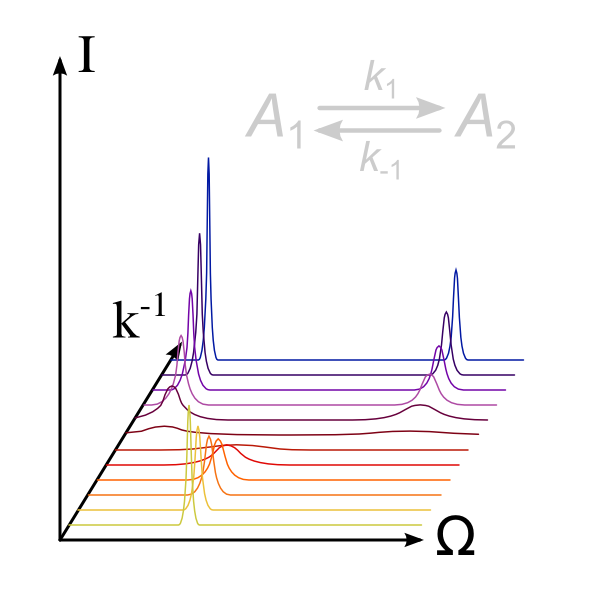
\includegraphics[width=5cm, bb=0 0 1701 1701]{graphics/analyses/relax_disp_600x600}
\end{figure*}


% Introduction.
%%%%%%%%%%%%%%%

\section{Introduction to relaxation dispersion}

Relaxation dispersion is the modulation of chemical exchange relaxation through the NMR pulse sequence.  For the $\Ronerho$-type experiment in which the nucleus of interest is spin-locked, either the spin-lock field strength or the offset between the spin-lock pulse and the chemical shift of the spins is modulated.  For the CPMG-type experiment, this time between the pulses is moduled.  Both experiment types are handled by relax.


% The models.
%~~~~~~~~~~~~

\subsection{The modelling of dispersion data}



% Script UI.
%%%%%%%%%%%%

\section{Analysing dispersion in the prompt/script UI mode}


% The sample script.
%~~~~~~~~~~~~~~~~~~~

\subsection{Dispersion script mode -- the sample script}


